\chapter[Softwareimplementering]{Software}

% Note om hvad der skal stå i dette afsnit her.


\section{Oversigt over softwaren}

% Her skriver vi hvordan softwaren er struktureret - se figuren nedenfor.

Softwaren er struktureret som vist i
figur\vref{fig:software-oversigt}. Dataføderen leverer data til den
del af softwaren, der behandler HPGL. Dataen kommer fra et
SD-kort. HPGL-behandleren sender instruktioner videre til den del af
motorkontrollen, der afvikles når der er tid. Denne del sætter
instruktioner i kø til realtidsdelen.

Realtidsdelen af motorkontrollen behandler de instruktioner, den anden
del af motorkontrollen har sat i kø og styrer stepmotorer m.m. efter
disse instruktioner. Realtidsdelen af motorkontrollen har ansvar for,
at hastigheden af tegnehovedet kan styres præcist.


\begin{figure}[htbp]
  \centering
  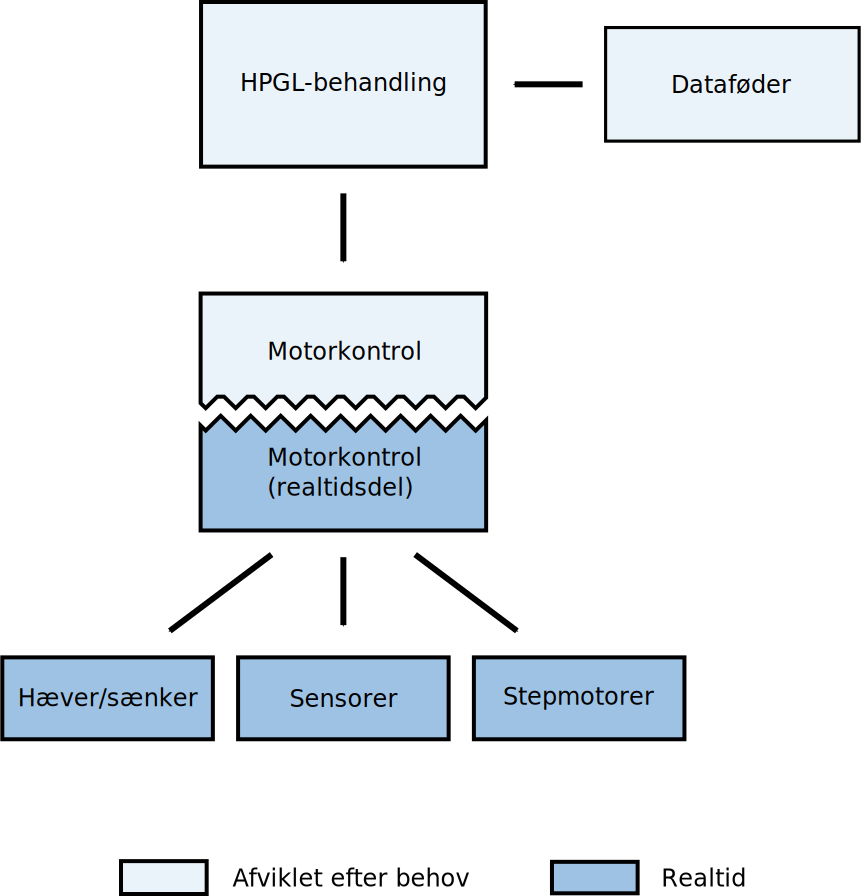
\includegraphics[width=.75\textwidth]{../brugere/kjaergaard/software-oversigt}
  \caption{Oversigt over softwaren. De lyseblå dele afvikles når der
    er tid til det. Når det er tid til at afvikle de mørkeblå områder,
    afbrydes afviklingen af de lyseblå.}
  \label{fig:software-oversigt}
\end{figure}


\section[Dataføder (med SPI og SD-/MMC-kort)]{Dataføder}

% Hvordan virker dataføderen (herunder buffer, spi og sd/mmc)?

En oversigt over funktionsfordelingen\fixme{andet ordvalg} i
dataføreren\fixme{andet ordvalg} kan ses i
figur\vref{fig:software-spi-sd-oversigt}.

\begin{figure}[htbp]
  \centering
  \includegraphics[width=\textwidth]{../brugere/kjaergaard/datafeeder-oversigt}
  \caption{Diagram over funktionsfordeling i dataføderen.}
  \label{fig:software-spi-sd-oversigt}
\end{figure}

Kommunikationen med SD-kortet foregår gennem SPI'en.\fixme{afsnit skal
  skrives færdig}. En eksempel på en forespørgsel med tilhørende svar
kan ses i figur\vref{fig:software-spi-sd-handling}.

\begin{figure}[htbp]
  \centering
  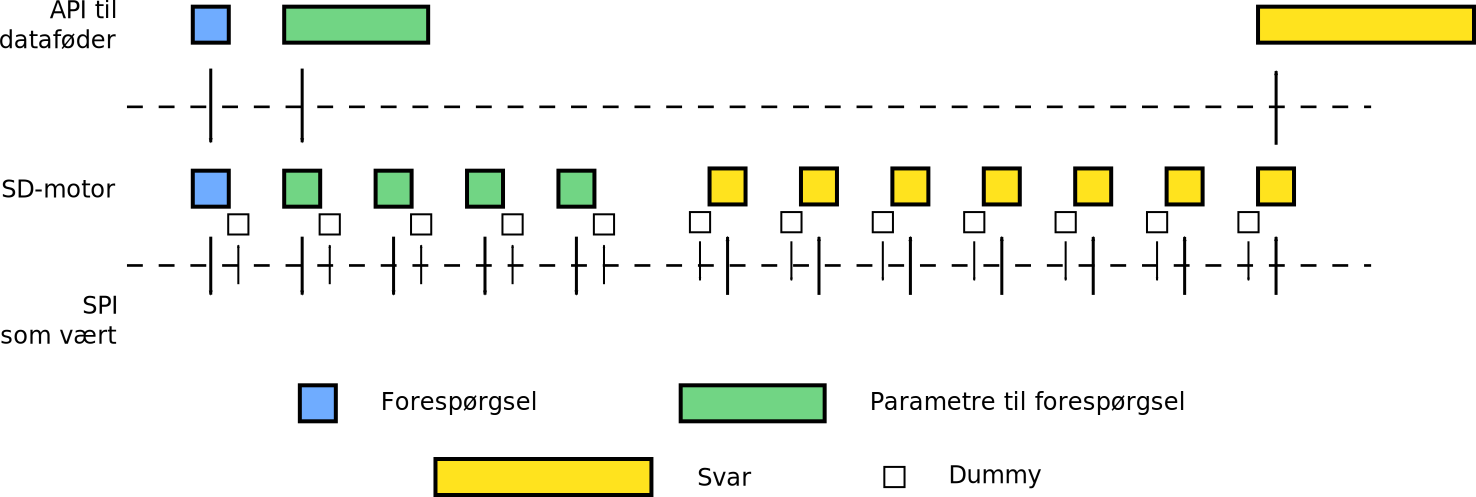
\includegraphics[width=\textwidth]{../brugere/kjaergaard/datafeeder-handling}
  \caption{Handlingdiagram ved kommunikation med SD-kortet.}
  \label{fig:software-spi-sd-handling}
\end{figure}


\section{HPGL-behandleren}

% Hvordan virker den del, der fortolker og behandler HPGL?


\section[Motorkontrol (med buffer)]{Motorkontrol}

% Hvordan er motorkontrollen implementeret? Beskriv implementeringen
% kort.


\section{Stepmotorstyring}

% Hvordan styres stepmotorerne? Superkort. Hvordan ser softwaren der
% styrer dem ud?


\section{Sensorer og løfter/sænker}


\section{HPGL -- Hewlett-Packard Graphics Language}

% Hvordan implementerer vi HPGL? Hvilke afvigelser tillader vi os at
% tage fra den dokumentation, vi har fundet?


%%% Local Variables: 
%%% mode: latex
%%% TeX-master: "../master"
%%% End: 